\chapter{Анализ и исследование стендовых и сгенерированных данных трафика и состояния сетей.}\label{ch:ch2}

\section{Данные Канадского Института Кибербезопасности(CIC)  }\label{sec:ch2/sec1}


Одной из важнейших задач в анализе трафика является его группировка по типу соединения, характеру содержимого и устройствам, участвующим в соединении. В связи с этим исследователи активно проводят эксперименты и сбор данных для данной задачи. Примером такой работы являются наборы данных Канадского Института Кибербезопасности (Canadian Institute for Cybersecurity - CIC). Эти наборы данных связаны с различным спектром задач: данные о передаваемых вредоносных файлах, зашифрованном и замаскированном трафике, а также типе передаваемых пакетов (мультимедия, переписка, передача файлов и др.).

Рассмотрим следующие наборы данных, упоминаемый в различных  научных исследованиях:

\begin{itemize}
	\item набор данных зашифрованного и незашифрованного трафика ISCXVPN (2016) \cite{icissp16}
	
	\item ISCXTor2016 — данные о трафике в сети ToR \cite{tornontor}
	
	\item набор данных CCCS-CIC-AndMal (2020), связанный с задачей классификации ПО на множество категорий и семейств вредоносных программ. \cite{Rahali2021}
	
\end{itemize}


Набор данных ISCXVPN нацелен на выявление особенностей, позволяющих различить VPN и не-VPN соединения.  В нем собраны различные статистики для различных значений временного окна: 15, 30, 60 и 120 секунд. В качестве исследуемых признаков представлены: 
\begin{itemize}
	\item Среднее количество пакетов в секунду
	\item Количество передаваемой информации (в килобайтах за секунду)
	\item Длительность соединения
	\item Различные статистики данных признаков в сторону исходного и конечного узла (среднее, максимум, минимум и т.п.). 
\end{itemize}
Также стоит подчеркнуть, что данные содержат различный спектр типов соединений :

\begin{itemize}
	\item Просмотр веб-страниц: HTTP и HTTPS трафик, генерируемый пользователями в браузерах (Firefox и Chrome).
	\item Чат: Трафик из приложений мгновенного обмена сообщениями, таких как Facebook, Hangouts через веб-браузер, Skype и ICQ с использованием приложения pidgin.
	\item Email: SMPTS, POP3S and IMAPS
	\item Аудио-стриминг: Трафик от приложений для потокового аудио, таких как Spotify.
	\item Видео-стриминг: Трафик от видеосервисов, таких как YouTube и Vimeo.
	\item FTP: Трафик для передачи файлов через Skype, SFTP и FTPS.
	\item VoIP: Трафик голосовых вызовов через Facebook, Hangouts и Skype.
	\item P2P: Трафик от протоколов обмена файлами (например, Bittorrent), собранный с использованием приложения Vuze.
\end{itemize}

Таким образом данные покрывают широкий спектр современных типов трафика, исключая смещений в картине распределения используемых признаков. Баланс классов изображен на рисунке \ref{fig:vpn_balance}

\begin{figure}[ht]
	\centerfloat{
		
\includegraphics[scale=0.6]{CIC/vpn_balance}
	}
	\caption{Баланс VPN и не-VPN трафика в наборе данных ISCXVPN(2016)}\label{fig:vpn_balance}
\end{figure}

ISCXTor2016 — это датасет, разработанный Университетом Нью-Брансуика, который представляет собой набор сетевого трафика, собранного для анализа различий между трафиком, проходящим через сеть Tor, и обычным интернет-трафиком. Этот датасет предназначен для исследователей в области кибербезопасности и сетевого анализа. Среди его особенностей стоит упоменять следующее:

\begin{itemize}
	\item Объем данных: Датасет содержит 22 ГБ данных, собранных с использованием инструментов Wireshark и tcpdump.
	
	\item Форматы данных: Включает полные пакеты в формате .pcap и CSV-файлы, созданные с помощью ISCXFlowMeter, который извлекает потоки из .pcap файлов.
\end{itemize}

Основным нюансом, усложняющим задачу классификации является сильный дисбаланс классов (Рисунок \ref{fig:tor_balance}). Также стоит отметить особенности в распределении используемых портов для соединений из сети Tor (Рисунок \ref{fig:nontor_port2}), что может свидетельствовать о некачественно сборе данных. Данный аспект может привести к плохой обобщаемости получаемых моделей.

\begin{figure}[ht]
	\centerfloat{
		
\includegraphics[scale=1.0]{CIC/tor_balance}
	}
	\caption{Баланс Tor и не-Tor трафика в наборе данных ISCXTor2016}\label{fig:tor_balance}
\end{figure}


\begin{figure}[ht]
	\centerfloat{
		
\includegraphics[width=\textwidth]{CIC/tor_port_balance}
	}
	\caption{Баланс используемых портов отправителем в данных Tor сетей ISCXTor2016}\label{fig:nontor_port2}
\end{figure}

В наборе данных CCCS-CIC-AndMal-2020 представлены различные характеристики о передаваемых по сети вредоносных файлах. Данный датасет сосредоточен на классификации вредоносных программ для Android, разработан в сотрудничестве между Канадским институтом кибербезопасности (CIC) и Университетом Нью-Брансуика. Этот датасет примечателен своим размером и разнообразием, содержащим 400 000 приложений для Android — 200 000 доброкачественных и 200 000 образцов вредоносных программ. Вредоносные образцы классифицированы на 14 различных категорий, включая рекламные баннеры (adware), программы-вымогатели, трояны и другие, охватывающие в общей сложности 191 семью вредоносных программ. Баланс упомянутых категорий программ представлены в Таблицу \ref{tab:malware_families}


\begin{table}[htbp]
	\centering
	\caption{Количественное описание изучаемых данных по категориям вредоносных программ}
	\begin{tabular}{|>{\centering}p{6cm}|>{\centering}p{4cm}|c|}
		\hline
		\textbf{Категория} & \textbf{Количество семейств} & \textbf{Количество образцов}                    \\ \hline
		Рекламоносители (Adware)                    & 48                       & 47\,210                     \\ \hline
		Бэкдор (Backdoor)                           & 11                       & 1\,538                      \\ \hline
		Программы-вымогатели (Ransomware)           & 8                        & 6\,202                      \\ \hline
		Троян (Trojan)                              & 45                       & 13\,559                     \\ \hline
		Троян-Банкир (Trojan-Banker)                & 11                       & 887                        \\ \hline
		Троян-Дроппер (Trojan-Dropper)              & 9                        & 2\,302                      \\ \hline
		Троян-SMS (Trojan-SMS)                      & 11                       & 3\,125                      \\ \hline
		Тролян-Шпион (Trojan-Spy)                   & 11					   & 3\,540				        \\ \hline
		Вирус нулевого дня (Zero-Day)               & -                        & 13\,340                     \\ \hline
		Файловый вирус (FileInfector)			    & 5     				   & 669 						\\ \hline
		Потенциально нежелательное приложение (PUA) & 8     				   & 6\,202					    \\ \hline
		ПО с потенциальным риском (Riskware)		& 21   					   & 97\,349  					\\ \hline
		Пугающее ПО (Scareware)						& 3    					   & 1\,556						\\ \hline
		Без категории				      			& -						   & 2\,296 						\\ \hline
	\end{tabular}
	\label{tab:malware_families}
\end{table}

Датасет CCCS-CIC-AndMal-2020 в первую очередь используется для академических исследований в области кибербезопасности, особенно для разработки моделей машинного обучения и глубокого обучения для обнаружения и классификации вредоносных программ. Он служит ценным ресурсом для тестирования новых алгоритмов и улучшения существующих методов обнаружения.

Далее описываются популярные методы и подходы, применяемые к анализу трафика и вредоносных приложений. Наборы данных ISCXVPN и ISCXTor2016 были опубликован в 2016 году и быстро стали довольно популярным в исследовательском сообществе. На момент 2024 года ISCXVPN имеет более 600, а набор ISCXTor2016 более 200 ссылок согласно системе Google Scholar. Датасет же CCCS-CIC-AndMal является более новым и пока не так тщательно изучен и имеет менее 100 ссылок в той же системе. 

Ниже представлены основные методы и подходы, представленные в современных научных трудах, которые используются для анализа сетевого трафика и обнаружения вредоносных приложений. Описанные ранее наборы данных ISCXVPN и ISCXTor2016, опубликованные в 2016 году, получили широкое распространение в научном сообществе и к 2024 году насчитывают более 600 и 200 цитирований соответственно по данным Google Scholar. В то же время датасет CCCS-CIC-AndMal является более современным, однако на данный момент изучен в меньшей степени и имеет менее 100 цитирований в той же системе. Наряду с работами, основанными на этих наборах данных, будут также в вкратце описаны работы, которые были протестированы на других данных, но решающие схожие задачи. В частности, будут описаны и методы предварительной обработки признаков, которые концептуально похожи на исследуемые в данной работе подходы.


Выбор наиболее объективного метода сравнения моделей машинного обучения — включая классические алгоритмы, глубокие нейронные сети (DNN) и ансамблевые подходы — может представлять определённые сложности и не всегда очевиден, даже при неизменности набора данных. В задачах классификации широкое распространение получили такие метрики качества, как accuracy (точность), precision (точность), recall (полнота) и F1-метрика (F1-score), которые систематически используются в большинстве исследовательских работ, рассматриваемых в данном контексте. Тем не менее, следует отметить, что метрика accuracy обладает существенным ограничением: её репрезентативность существенно снижается в условиях несбалансированности классов, поскольку она не учитывает диспропорции в их распределении. В связи с этим, её применение оправдано лишь при условии приблизительно равного представления классов в выборке. Особо подчеркнём, что описанные выше наборы данных характеризуются выраженной несбалансированностью классов. Несмотря на это, в ряде научных публикаций оценка качества моделей ограничивается исключительно значением accuracy, без представления дополнительных, более информативных метрик. Формулы и определения используемых метрик приведены в Таблице \ref{tab:metrics}.


\begin{table}[h]
	\centering
	\caption{Метрики качества для задачи классификации}
	\label{tab:metrics}
	\begin{tabular}{|>{\centering\arraybackslash}p{3cm}|>{\centering\arraybackslash}p{5.5cm}|>{\centering\arraybackslash}p{6cm}|}
		\hline
		Метрика & Формула & Описание \\
		\hline
		\rule{0pt}{4ex}
		Accuracy (Точность) & 
		$\dfrac{TP + TN}{TP + TN + FP + FN}$ &
		Доля правильных предсказаний модели среди всех сделанных предсказаний. \\
		
		\hline
		\rule{0pt}{4ex}
		Precision (Точность) & 
		$\dfrac{TP}{TP + FP}$ &
		Доля истинно положительных предсказаний среди всех положительных предсказаний модели. \\
		
		\hline
		\rule{0pt}{4ex}
		Recall (Полнота) & 
		$\dfrac{TP}{TP + FN}$ &
		Доля истинно положительных предсказаний среди всех реально положительных случаев. \\
		
		\hline
		\rule{0pt}{4ex}
		F1-метрика & 
		$2 \times \dfrac{\text{Precision} \times \text{Recall}}{\text{Precision} + \text{Recall}} = \dfrac{2 \cdot TP}{2 \cdot TP + FP + FN}$ &
		Гармоническое среднее между точностью и полнотой, учитывает обе метрики. \\
		\hline
	\end{tabular}
\end{table}


Современные методы классификации сетевого трафика в основном опираются на статистические подходы, включая методы машинного обучения и глубокие нейронные сети. Наиболее распространены методы анализа <<полезной нагрузки>> пакетов — так называемые технологии Deep Packet Inspection (DPI) \cite{Fang2006} и Deep Flow Inspection (DFI) \cite{Meiners2012}, которые основаны на выявлении характерных шаблонов посредством частотного анализа сигнатурных признаков. Однако данные методы демонстрируют ограниченную эффективность при анализе зашифрованного или обфусцированного (замаскированного под обычный) трафика, что существенно снижает их точность \cite{Bregni2010}. Например, адаптация DPI, предложенная в работе \cite{Sherry2015}, показала лишь 91\% точности при классификации HTTPS-трафика, что указывает на недостаточную устойчивость подхода к современным протоколам шифрования.

Рассмотрим некоторые альтернативные методы, в частности те, что использовали вышеописанные наборы данных. В исследовании \cite{icissp16} представлена методология сбора и обработки данных ISCXVPN, а также продемонстрированы высокие показатели эффективности: достигнуты значения точности и полноты на уровне 90\% в задаче бинарной классификации (разделение на VPN и non-VPN). Кроме того, авторы рассматривали сценарий одновременного обнаружения зашифрованного и открытого трафика, а также идентификации приложений в обоих типах потоков (для сценария B), где среднее значение accuracy составило 84\%, что подтверждает перспективность данного подхода при анализе гетерогенного трафика.

Другим перспективным направлением является предварительная обработка сетевых данных с применением кластеризации и ансамблевых моделей. Данный подход основывается на гипотезе о существовании нескольких независимых источников (генераторов) трафика, каждый из которых характеризуется уникальным статистическим распределением. Разделение данных на кластеры, соответствующие отдельным генераторам, позволяет построить специализированные классификационные модели для каждого кластера, что повышает общую точность распознавания. Ярким примером реализации такой стратегии служит ансамбль моделей гауссовских процессов (Gaussian Process Regression, GPR), предложенный в \cite{Bayati2020}, который демонстрирует высокую эффективность в условиях сложной структуры трафика.

Одним из широко применяемых методов в анализе сетевого трафика является наивный байесовский классификатор (Naive Bayes), который используется благодаря своей вычислительной эффективности и устойчивости к переобучению \cite{Athanasios2019, Sharafaldin2018TowardGA}. В работе \cite{moore2005} предложена модифицированная версия данного алгоритма, позволяющая достичь accuracy для классификации до 95\%, что подчеркивает потенциал вероятностных моделей в данной предметной области.

Эволюционный вычислительный подход также был изучен в задачах сетевого анализа. Так, в работе \cite{Fernando2015} авторами был использован подход с методом конкурентного отбора ENORA, который позволил достичь F1-метрики 0,95–1,0 в различных сетевых приложениях.

Следует отметить исследования, посвящённые применению методов понижения размерности признакового пространства в контексте анализа сетевого трафика. В работе \cite{Saber2019} для предварительной обработки данных использовался линейный дискриминантный анализ (LDA) в качестве метода снижения размерности. Авторы достигли значения метрики accuracy на уровне 0,98, однако в публикации отсутствует детализация относительно параметров настройки LDA, характеристик полученного уменьшенного признакового пространства, а также описания экспериментальной методологии, что затрудняет воспроизведение и оценку результатов.

В исследовании \cite{Manju2019} предложен подход к отбору признаков, основанный на анализе важности признаков в рамках ансамбля деревьев решений. В качестве базового метода оценки значимости использовалась частота вхождения признаков в структуру деревьев, что является распространённой эвристикой для определения информативности признаков. На следующем этапе применялся алгоритм экстремального градиентного бустинга (XGBoost из библиотеки XGB) для построения модели и последовательного добавления признаков в порядке убывания их важности. При каждом добавлении нового признака производилась оценка точности модели, и процесс продолжался до достижения плато в значении метрики accuracy, что интерпретировалось как определение оптимального подмножества признаков. Данный подход позволил сократить размерность признакового пространства с исходных 248 признаков до 8, сохранив при этом высокую классификационную эффективность. В результате было зафиксировано увеличение метрики accuracy на 6\% по сравнению с базовыми моделями. Отмечается, что подобный метод может демонстрировать более выраженные преимущества в условиях несбалансированных выборок, хотя данное утверждение требует дополнительной эмпирической проверки. Эксперименты проводились на стандартных датасетах, предоставленных Кембриджским университетом, что обеспечивает определённую степень сопоставимости результатов с другими исследованиями в данной области.


В другой работе \cite{Haitham2019} авторы сравнили различные алгоритмы отбора признаков, такие как хи-квадрат, информационный прирост, коэффициент прироста, анализ главных компонент (PCA) и другие. Лучший набор признаков был выбран на основе пяти алгоритмов машинного обучения: HoeffdingTree, J48, SMO, метод опорных векторов (SVM) и наивный байесовский метод. Исследуя трассировки трафика UNIBS из наборов данных Университета Брешии и Кембриджа \cite{unibs} , авторы достигли метрики accuracy до 99,799\% с помощью PCA и J48.


Ручная инженерия признаков представляет собой ресурсоёмкий и трудозатратный процесс при разработке моделей машинного обучения, поскольку требует значительных усилий специалистов по данным и глубоких предметно-ориентированных знаний. Кроме того, данный подход характеризуется ограниченной обобщаемостью, поскольку набор релевантных и информативных признаков может существенно варьироваться в зависимости от предметной области и специфики решаемой задачи. В связи с этим всё большее распространение получают методы автоматического извлечения признаков, основанные на архитектурах глубоких нейронных сетей, которые способны выявлять сложные нелинейные зависимости в данных без необходимости явного задания признаков вручную. Так, в работе \cite{Haitham2019} предложена модель Deep Packet, сочетающая архитектуру автоэнкодера (autoencoder) и свёрточной нейронной сети (CNN) для одновременного извлечения признаков и классификации сетевого трафика. Автоматическое извлечение признаков на ранних слоях сети позволяет модели эффективно работать с сырыми или слабо предобработанными данными, минимизируя зависимость от ручного проектирования признаков. Авторы демонстрируют высокую эффективность подхода, достигнув значения F1-меры на уровне 0,91, что подтверждает перспективность использования глубоких архитектур в задачах анализа трафика.

Также стоит упомянуть работу \cite{Ma2020}, где представлена модификация K-nn -- алгоритм взвешенных k-ближайших соседей (Weighted k-Nearest Neighbors, WKNN), который продемонстрировал accuracy вплоть до 0,99 для задачи бинарной классификации трафика на наборе данных ISCXVPN. В рамках данной работы был разработан самоадаптивный алгоритм отбора признаков (WKNN-Selfada), в котором веса признаков динамически определяются в процессе обучения. Веса интегрируются в метрику взвешенного расстояния Минковского, где их величина отражает вклад соответствующего признака в разделение объектов различных классов. Основная гипотеза метода заключается в том, что признаки, демонстрирующие большее межклассовое расстояние, обладают более высокой дискриминативной способностью и, следовательно, должны иметь больший вес в расчёте сходства. Предложенный подход обеспечивает адаптацию классического KNN к условиям зашифрованного трафика, где традиционные признаки могут быть менее информативны, а распределения данных — более сложными для разделения.

%%%%%%%%%%%%%%%%

Рассмотрим также вторую задачу, связанную с использованием набора данных CCCS-CIC-AndMal-2020, который предназначен для обнаружения вредоносного программного обеспечения в экосистеме Android. Рост популярности мобильных устройств на платформе Android сопровождается значительным увеличением количества и сложности вредоносных приложений, что обуславливает необходимость разработки эффективных методов их анализа и классификации.

Методы анализа вредоносного ПО традиционно подразделяются на два основных подхода: статический и динамический анализ. Статический анализ предполагает извлечение признаков на основе структурных и семантических характеристик приложения без его исполнения, включая анализ манифест-файлов, байт-кода, вызовов системных API и графа вызовов. Данный подход позволяет быстро обрабатывать большое количество приложений, однако он уязвим к методам обфускации кода. Динамический анализ, напротив, основан на мониторинге поведения приложения в контролируемой среде выполнения (песочнице), что позволяет фиксировать его взаимодействие с системными ресурсами, сетевыми соединениями и аппаратными компонентами. Этот метод более устойчив к обфускации, но требует значительных вычислительных ресурсов и времени на сбор данных.

В ряде исследований, включая работу \cite{Yuan2014}, демонстрируется перспективность гибридного подхода, объединяющего преимущества обоих методов. Комбинирование статических и динамических признаков позволяет повысить полноту представления поведения приложения и улучшить качество классификации, особенно в условиях сложных и эволюционирующих угроз.


Классические методы машинного обучения, такие как метод опорных векторов (Support Vector Machine, SVM), дерево решений (Decision Tree, DT), алгоритм k-ближайших соседей (k-Nearest Neighbors, KNN) и наивный байесовский классификатор (Naive Bayes, NB), активно применяются для задачи обнаружения вредоносного программного обеспечения для операционной системы Android \cite{Zhang2014, Cai2019}. Эти подходы демонстрируют высокую эффективность при анализе статических и поведенческих признаков приложений, что делает их популярным выбором в ряде исследований. В то же время, с развитием технологий глубокого обучения, всё большее распространение получают нейросетевые подходы. В частности, для детекции вредоносных приложений используются глубокие вероятностные модели, такие как глубокая сеть доверия (Deep Belief Network, DBN), построенная на основе стекинга ограниченных машин Больцмана (Restricted Boltzmann Machines, RBM), а также детерминированные архитектуры — свёрточные нейронные сети (Convolutional Neural Networks, CNN) и рекуррентные сети с долгой краткосрочной памятью (Long Short-Term Memory, LSTM) \cite{Yuan2014, Hou2016, Nix2019}. Указанные модели позволяют эффективно обрабатывать как структурированные, так и последовательные данные, что повышает точность классификации в условиях сложных и динамически изменяющихся угроз.


Сами авторы набора данных CCCS-CIC-AndMal-2020 \cite{Rahali2021} применили алгоритм Extremely Randomized Trees Classifier (ExtraTreesClassifier) \cite{extra_tree} для выбора наиболее релевантных признаков. Признаки были отобраны на основе нормализованного общего снижения важности Джини. Авторы преобразуют признаки, извлеченные из файлов APK, в 2D-изображения. После этого шага признаки были переданы в CNN. В ходе экспериментов авторы достигли accuracy 93,36\% для задачи характеристики вредоносного ПО для Android.


Здесь следует упомянуть несколько интересных подходов к проектированию признаков в контексте вредоносных приложений Android. Один из них был предложен в \cite{Huang2018}, в данном методе автоматизировали извлечение признаков путем преобразования байт-кода приложения Android в цветовой код Red, Green, Blue (RGB). После чего полученные изображения использовались в качестве входных данных для сверточной нейронной сети.

%В работе \cite{KARBAB2018} представили MalDozer - систему обнаружения и атрибуции вредоносных программ для Android. Эта система извлекает необработанные последовательности вызовов API из кода сборки и использует эти данные в качестве входных данных для CNN.

Другие исследователи уже исследовали этот набор данных и предложили несколько решений для задачи. Одно из них - EntropLyzer \cite{Keyes2021}. Авторы классифицируют категории вредоносного ПО используя классические модели машинного обучения: алгоритм случайного леса (RandomForest, RF), наивный байесовский классификатор (NB) и решающее дерево (DT). Так, для RF они достигли precision 0,769, а для  DT - precision достигла 0,984.

Также были исследованы и архитектуры глубоких нейросетей. Например, в работе DIDroid \cite{Rahali2021} исследователи использовали модель, которую назвали Deep Image Learning. Авторы использовали 15-слойную DNN и получили довольно высокую производительность. В ходе тестирования они достигли accuracy более 93\%.

Перечисленные результаты будут использованы для последующего сравнительного анализа исследуемых методов обработки данных.


\section{Применение методов генерации признаков в задачах анализа трафика }\label{sec:ch2/sect2}

В данном разделе приведены основные результаты по задаче анализа трафика. Для исследования эффективности методов использовались описанные выше наборы данных от института CIC.


\subsection{Применение метода AGMV}\label{sec:ch2/sect2/sub1}

Одним из исследуемых методов был метод генерации признаков - Accumulated Generelized Mean Value (AGMV). 

Предположим, что есть временной ряд для признака $F_{j}$ который обозначим как $x_{j}(t_{i})$, где $t_{i}$ - $i$-ый момент времени, где $j \in \{1,..., P\}$, $i \in \{0, 1, ..., N-1\}$, $P$ - количество признаков, $N$ - количество рассматриваемых временных отсчетов $t_i$. Тогда запись для AGMV будет выглядеть следующим образом:

\begin{equation}\label{eq:one}
	AGMV (x_j (t_i), p, a, K, M) = \left \{ \frac{1}{M-K}\sum_{i=K, i = i + a}^{M-1} (\left | x_j(t_i) \right |^{p}) \right \} ^{1/p},
\end{equation}
где $x_j$ — значения временного ряда для признака $F_j$ на интервале индексов [K, M], а соответственно (M - K) — длинна анализируемого окна $w$, $a$ — параметр децимации (другими словами, параметр, регулирующий шаг вычислений. При $a=1$ используется все имеющиеся точки, а для $a=2$  используется каждая вторая), а $p$ — параметр, управляющий чувствительностью метода.

Итак, как указано выше - параметр $p$ соответствует чувствительности метода. Исследования показывают, что временные ряды в наборе данных могут требовать различных оптимальных значений чувствительности $p$, а также других параметров (см. \cite{Ivch_2021}). %*(Рисунок~\ref{fig2}). 
Идея этого подхода основана на предположении, что различные классы данных, которые описываются набором временных рядов, имеют различное поведение последовательностей, например, на их стыках есть всплески или разрывы. Функция \ref{eq:one} нацелена на оценку переходов из одного класса в другой и зависит от различий их характеристик.

Меняя параметр чувствительности рассматриваемый метод можно преобразовать в широко известные математический функции, в частности геометрическое, гармоническое и арифметическое средние. Более подробную информацию можно найти в \cite{Ivch_2021}. Подход AGMV производит отображение признаков $x_j(t_i)$ в признаки $x_l'(t_i)$. Стоит отметить, что метод применяется не для всех данных, а отдельно для каждого окна размером $w \le N$ отдельно. Для каждого блока вычисляется функция (\ref{eq:one}) и используется как новые признаки. 


В предыдущих исследованиях \cite{Ivch_2021} была предложена реализация метода AGMV для анализа сетевого трафика в ходе работы с набором данных ISCXVPN \cite{icissp16}. Были выставлены следующие параметры: длина шага $a=1$, чувствительность на уровне $p=0,1$ и  размер окна $w=500$. С помощью  нескольких распространенных алгоритмов машинного обучения, реализованных в библиотеке scikit-learn, и рандомизированного поиска гиперпараметров с использованием кроссвалидации (cross-validation) были достигнуты результаты, сравнимые с аналогами прис условии использования относительно простого метода предобработки (Таблица \ref{tab:sota_agmv}).


\begin{table}[h] 
	\centering
	\caption{ Сравнение результатов базовой версии AGMV  (* не упомянуто; ** Accuracy составила 99\% ; Pr - Precision, Rc - Recall)}
	\begin{tabular}{|>{\centering\arraybackslash}p{4cm}|c|c|c|c|c|c|}
		%\br
		%\textbf{Method}	& \textbf{Scenario A1}	& \textbf{Scenario A2} & \textbf{Scenario A3}\\
		\hline
		\multirow{2}{*}{\textbf{Метод}} & \multicolumn{2}{c|}{\textbf{Сценарий A1}} & \multicolumn{2}{c|}{\textbf{Сценарий A2}} & \multicolumn{2}{c|}{\textbf{Сценарий B}} \\
		\cline{2-7}
		&    Pr     &     Rc   &    Pr     &    Rc    &    Pr     &    Rc    \\
		\hline
		WKNN \cite{Ma2020}   &   **      &   **     &   0,936   &   0,945  &    *      &   *      \\
		\hline
		Decision tree + AGMV \cite{Ivch_2021}  &\textbf{0,989} & \textbf{0,989} & \textbf{0,990}&\textbf{0,987}&\textbf{0,986 } & \textbf{0,984}\\
		\hline
		Gil et al. \cite{icissp16}, C4.5  &  0,89   &   0,91    &  0,84    &  0,89    &  0,84     &    *     \\
		\hline
		Deep Packet \cite{Lotfollahi2019}, CNN &   *       &     * &     *  &    *  &    0,94       &    0,94  \\
		\hline
		%\br
	\end{tabular}
	\label{tab:sota_agmv}
\end{table}



Используя простой постоянный набор параметров AGMV, была получена функция преобразования признаков. При этом значения начинают вычисляться заново в каждом окне $w$. Но можно отметить, что на границе между классами мы наблюдаем сохранение поведения признаков.


%%%% my res

Было обучено 4 модели для задачи бинарной классификации (данные VPN/nonVPN, сценарий A1): Случайный лес (Random Forest (RF)), классическое дерево решений (DT), градиентный бустинг XGBoost (XGB) и классификатор на методе опорных векторов (Support Vector Machine (SVM)). AGMV использовался с параметрами «по умолчанию» согласно работе \cite{Ivch_2021}: размер окна $w=400$, чувствительность $p=1$, децимация $a=1$, также окна использовались без наложения. При использовании AGMV с данными значениями параметров была достигнута accuracy  более 0,95 с использованием модели RF (Рисунок \ref{fig:vpn_best}). Но главное -  метод AGMV дает значительное увеличение производительности (Рисунок \ref{fig:ISCXVPN_cv}) для всех протестированных моделей (Таблица \ref{vpn_res}).



\begin{figure}[h]
	\center{
\includegraphics[width=8 cm]{VPN_best_estimator.png}}
	\caption{Метрика accuracy для лучшей комбинации гиперпараметров для бинарной классификации с и без использования AGMV для набора данных ISCXVPN для алгоритма случайного леса (RandomForest)}
	\label{fig:vpn_best}
\end{figure} 

Из набора CCCS-CIC-AndMal-2020 использовалась часть данных, связанная с динамическим анализом (Dynamic Analysis) и были обучены те же 4 модели для задачи мультиклассовой классификации по оценке категорий вредоносного ПО. Оба сценария набора данных (до и после перезагрузки) имеют схожее поведение. Была также достигнута точность более 0,95 для нескольких моделей (Рисунок \ref{ar_acc_best}). Аналогичное исследование со сбором средних значений метрик accuracy, precision и recall для различных данных показывает, что AGMV демонстрирует свою эффективность для задач мультиклассовой классификации (Рисунок \ref{ar_acc_best}). Все результаты представлены в таблицах \ref{male_res} и \ref{male_pr_rc}.

\begin{figure}[h]
	\center{
\includegraphics[width=8 cm]{AR_Accuracy.png}}
	\caption{Метрика accuracy для лучшей комбинации гиперпараметров для мультиклассовой классификации с и без использования AGMV  для набора данных CCCS-CIC-AndMal (сценарий датасета Before reboot) для моделей случайного леса (RandForest), дерева решений (Tree), машины опорных векторов (SVM) и градиентного бустинга (XGB)}
	\label{ar_acc_best}
\end{figure}


\begin{figure}[h]
	\center{
\includegraphics[width=16 cm]{BR_Accuracy_boxplot_all_models.png}}
	\caption{Метрика accuracy для мультиклассовой классификации с и без использования AGMV, оцененная на кроссвалидации на 5 подвыборках для набора данных CCCS-CIC-AndMal (сценарий датасета Before reboot )}
	\label{malware_res_gr}
\end{figure}

% уже выводы 
Таким образом была продемонстрирована эффективность подхода AGMV к предварительной обработке признаков для данных в наборах ISCXVPN и CCCS-CIC-AndMal.С равнение и анализ производительности были проведены для 4 классических ML-моделей (Таблицы \ref{male_res} и \ref{male_pr_rc}).


Как было показано, AGMV позволяют достичь значений  accuracy более 0,95 в обеих задачах: бинарной классификации трафика и мультиклассовой категоризации вредоносных программ. Мы достигли таких же результатов, как и для передовых методов, но в некоторых случаях модели с использованием AGMV продемонстрировали более высоких показателей метрик эффективности. Тем не менее, видится необходимость в улучшении всех метрик, в частности чувствительных к дисбалансу классов. 


Одним из ограничений метода AGMV является зависимость характера обнаружения от значений параметров, в частности от размера окна. В дальнейших исследованиях предполагается изучить взаимосвязи между параметрами и поведением метода, с акцентом на связь с размером окна $w$ и параметром чувствительности 
$p$. Кроме того, в настоящей работе использовались признаки, уже извлеченные из исходных данных. В перспективе планируется применение метода AGMV к другим типам данных, включая сырые файлы. В заключение следует отметить, что в данной работе не проводится сравнение скорости обработки. Предполагается, что исследуемый подход окажется более эффективным по скорости по сравнению с DNN, однако для других методов требуется дополнительное детальное исследование.



\begin{figure}[ht]
	\centerfloat{
		
\includegraphics[width=0.9\textwidth]{CIC/ISCXVPN_cv}
	}
	\caption{Метрика accuracy для бинарной классификации для набора данных ISCXVPN с и без использования преобразования признаков, оцененная на кроссвалидации на 5 подвыборках}
	\label{fig:ISCXVPN_cv}
\end{figure}




\begin{table}[h] 
	\centering
	\caption{Средние показатели метрики accuracy для бинарной классификации для набора данных ISCXVPN}
	\begin{tabular}{|>{\centering\arraybackslash}p{2.2cm}|c|c|c|c|c|c|c|c|}
		%\br
		\hline
		Время & RF & DT & XGB & SVM & RF + & DT + & XGB + & SVM + \\
		потока, сек & & & & & AGMV & AGMV & AGMV & AGMV \\   
		\hline
		15 & 0,808 & 0,754 & 0,795 & 0,606 & 0,973 & 0,908 & 0,865 & 0,866 \\
		\hline
		30 & 0,797 & 0,747 & 0,782 & 0,607 & 0,984 & 0,914 & 0,943 & 0,847 \\
		\hline
		60 & 0,747 & 0,694 & 0,741 & 0,624 & 0,973 & 0,921 & 0,843 & 0,807 \\
		\hline
		120 &0,791 & 0,729 & 0,733 & 0,636 & 0,992 & 0,920 & 0,927 & 0,847 \\
		\hline
		%\br
	\end{tabular}
\label{vpn_res}
\end{table}




\begin{table}[h] 
	\centering
	\caption{Средние показатели метрики accuracy для мультиклассовой классификации на наборе данных CCCS-CIC-AndMal}
	\begin{tabular}{|l|l|l|l|l|}
		\hline
		\multicolumn{5}{|c|}{\textbf{Before reboot сценарий}} \\
		\hline
	 & \textbf{RF} & \textbf{DT} & \textbf{XGB} & \textbf{SVM} \\ 
		\hline
		\textbf{Базовые признаки} & 0,64 & 0,521 & 0,637 & 0,594 \\
		\hline
		\textbf{AGMV} & 0,937 & 0,8 & 0,945 & 0,927 \\
		\hline
		\multicolumn{5}{|c|}{\textbf{After reboot сценарий}} \\
		\hline
		\textbf{Базовые признаки} & 0,642 & 0,493 & 0,712 & 0,587 \\
		\hline
		\textbf{AGMV} & 0,924 & 0,814 & 0,916 & 0,895 \\
		\hline

	\end{tabular}
	\label{male_res}
\end{table}


\begin{center}
	\begin{table}[h] 
		\centering
		\caption{Средние значения метрик precision(Pr) и recall(Rc) для задачи мультиклассовой классификации на наборе данных CCCS-CIC-AndMal}
		\begin{tabular}{|>{\centering}p{4cm}|c|c|c|c|c|c|c|c|}
			\hline
			\multicolumn{9}{|c|}{\textbf{Cценарий <<Before reboot>> }} \\
			\hline
			 & \multicolumn{2}{c|}{\textbf{RF}} & \multicolumn{2}{c|}{\textbf{DT}} & \multicolumn{2}{c|}{\textbf{XGB}} & \multicolumn{2}{c|} {\textbf{SVM}} \\ 
			\hline
			& \textbf{Pr} & \textbf{Rc} & \textbf{Pr} & \textbf{Rc} & \textbf{Pr} & \textbf{Rc} & \textbf{Pr} & \textbf{Rc} \\
			\hline
			\textbf{Базовые признаки} & 0,691 & 0,384 & 0,379 & 0,26 & 0,735 & 0,481 & 0,607 & 0,372 \\
			\hline
			\textbf{AGMV} & 0,811 & 0,814 & 0,467 & 0,472 & 0,873 & 0,869 & 0,903 & 0,874 \\
			\hline
			\multicolumn{9}{|c|}{\textbf{Cценарий <<After reboot>>}} \\
			\hline
			\textbf{Базовые признаки} & 0,641 & 0,391 & 0,396 & 0,232 & 0,681 & 0,483 & 0,577 & 0,375 \\
			\hline
			\textbf{AGMV} & 0,811 & 0,79 & 0,467 & 0,544 & 0,873 & 0,811 & 0,903 & 0,779 \\
			\hline

		\end{tabular}
		\label{male_pr_rc}
	\end{table}
\end{center}


\subsection{Применение метода CapoNef}\label{sec:ch2/sect2/sub2}

Еще одним исследуемым методом генерации признаков был метод CapoNef. Его принцип несколько отличается от рассматриваемого ранее AGMV.
CAPoNeF (Comparative Analysis of the Positive and Negative Fluctuations) - также метод, которые производит анализ временных рядов. Его отличительной особенностью является то, что ряды в нем анализируются как бестрендовоые последовательности (trendless sequences (TLS)).

Суть метода заключается в извлечении признаков из временных последовательностей, при условии, что они являются бестрендовыми. Метод включает в себя среденее значение, а также ряд характеристик для отклонений значений ряда от среднего значения, такие как диапазон между положительными и отрицательными флуктуациями, баланс между ними и другие связанные с ними характеристики (Таблица \ref{tab:caponef}). Общая схема получения метрик из исходных данных отображена на Рисунке  \ref{fig:caponefgeneral}.

Метод был разработан в МФТИ и был впервые освящен в 2020 году. Данный метод уже показал свою высокую эффективность в задачах анализа уровня сахара в крови и радиометрической идентификации \cite{Nigmatullin2020, Nigmatullin2021}.

\begin{figure}[h]
	\centering
	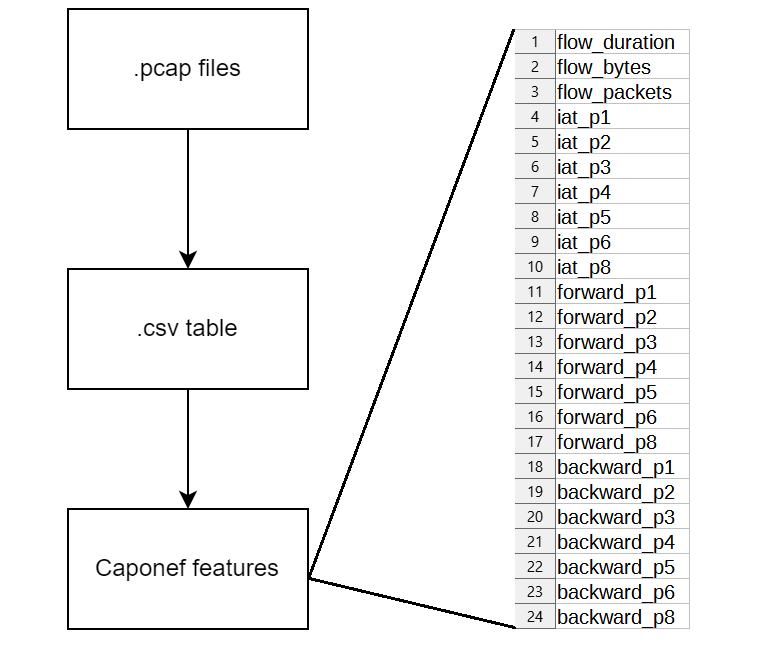
\includegraphics[width=0.7\linewidth]{images/caponef/caponef}
	\caption{Схема генерации признаков из исходных файлов}
	\label{fig:caponefgeneral}
\end{figure}



\begin{table}[h]
	\centering
	\caption{Описание использованных в работе методов генерации признаков (в формулах используется $Dy_i = y_i -<y>$)}
	\begin{tabular}{|>{\centering\arraybackslash}p{3cm}|>{\centering\arraybackslash}p{6cm}|>{\centering\arraybackslash}p{7cm}|}
		\hline
		Обозначение & Формула & Описание \\ 
		\hline
		$p_1$ & $<y>$ & арифметическое среднее \\
		\hline
		$p_2$ & $max(Dy_i) - min(Dy_i)$ & размах всех флуктуаций \\
		\hline
		$p_3$ & $max(Dy_i^+) - |min(Dy_i^-)|$ & баланс между максимальными положительными и отрицательными колебаниями \\
		\hline
		$p_4$ & $max(J_{up})- min(J_{dn})$ & максимальная кумулятивная интенсивность между положительными и отрицательными колебаниями ( $J_{up}, J_{dn}$ соответствуют суммам, взятым от исходных последовательностей $y_j$)\\
		\hline
		$p_5$ & $ \dfrac{[max(y_i)-mean(y_i)]}{[mean(y_i)-min(y_i)]}$ & мера асимметрии \\
		\hline
		$p_6$ & $N(Dy_i^+)-N(Dy_i^-)$ & показатель симметрии  кол-ва положительных и отрицательных  флуктуаций \\
		\hline
		$p_8$ & $Range[J(y_n)]$ & $y_n = (y - <y>)/Range(y)$, $Range(y_n)=1$, где $Range(f)=max(f)-min(f)$ \\
		\hline
	\end{tabular}
	\label{tab:caponef}
\end{table}




В работе сравнивались два набора признаков: Первый — базовые признаки, уже включенные в данные авторами данного датасета, а также признаки согласно методу CAPoNeF, полученные путем обработки исходных данных трафика в формате файлов .pcap.  Таким образом, можно заметить, что признаковое пространство значительно увеличилось. На этих данных было обучено два алгоритма: это Случайный лес из библиотеки <<sci-kit learn>>,  а также градиентный бустинг  из бибилиотеки XGB. В задаче бинарной классификации на данных VPN/non-VPN трафика удалось получить значение точности вплоть до 0,8, но к сожалению рассматриваемый метод не показал себя более эффективным по сравнению с базовым набором признаков(на графиках он обозначен как IAT). Результаты работы метода показаны на Рисунке  \ref{fig:capo}.

Исходя из вклада признаков в предсказывание категории трафика можно сделать вывод, что модель обобщилась хорошо, но к сожалению данный метод оказался не столь эффективным для рассматриваемой задачи. То есть для задачи классификации VPN трафика для данных со структурой, представленной в наборе ISCXVPN, метод CAPoNeF оказался не эффективен, особенно с учетом того, что размерность признакового пространства кратно увеличилась (7 метрик против изначальных 4) по сравнению с базовым набором (IAT). Однако это не исключает потенциальную эффективность для других задач обработки трафика, а также эффективность для данных с иной структурой. Поэтому в дальнейшем исследовании планируется проделать более детальное исследование данного метода, тестирование для других задач и наборов данных с отличной от уже рассмотренной структурой


Итак, была проведен анализ  метода извлечения признаков для задачи анализа интернет-трафика. Хоть в целом метода показал себя работоспособным  и полученная метрика показывает, что модели работают лучше, чем генератор случайных чисел (ГСЧ). Но тем не менее значимых приростов в показателях не наблюдалось при условии значительного увеличения кол-ва признаков. Поэтому следует провести тестирование для других задач и наборов данных с отличной от уже рассмотренной структурой. Тем не менее результаты указывают на то, что поиск и тестирование стоит сместить в сторону других альтернативных методов, которые приведут к повышению точности в рассмотренных задачах.

\begin{comment}
\begin{figure}[ht]
	\centering
	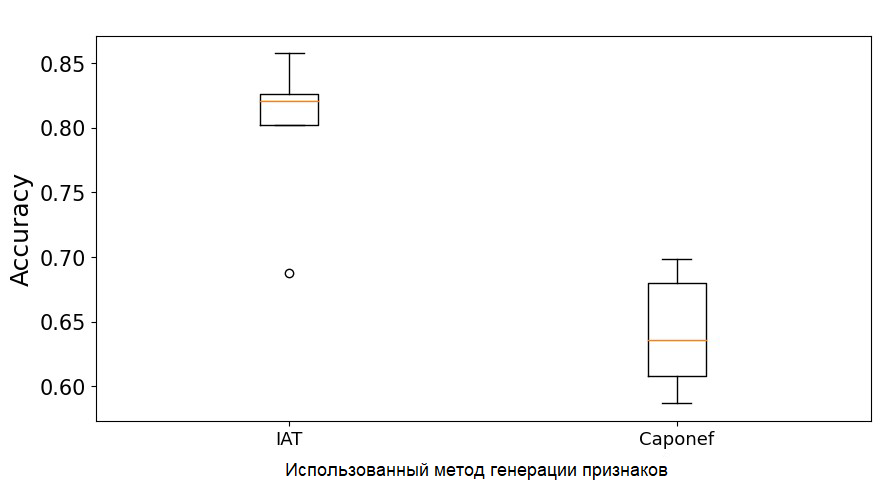
\includegraphics[width=0.9\linewidth]{images/caponef/xgb}
	\caption{Результаты использование CAPoNeF и алгоритма градиентного бустинга для задачи бинарной классификации набора данных ISCXVPN}
	\label{fig:xgb}
\end{figure}

\begin{figure}[ht]
	\centering
	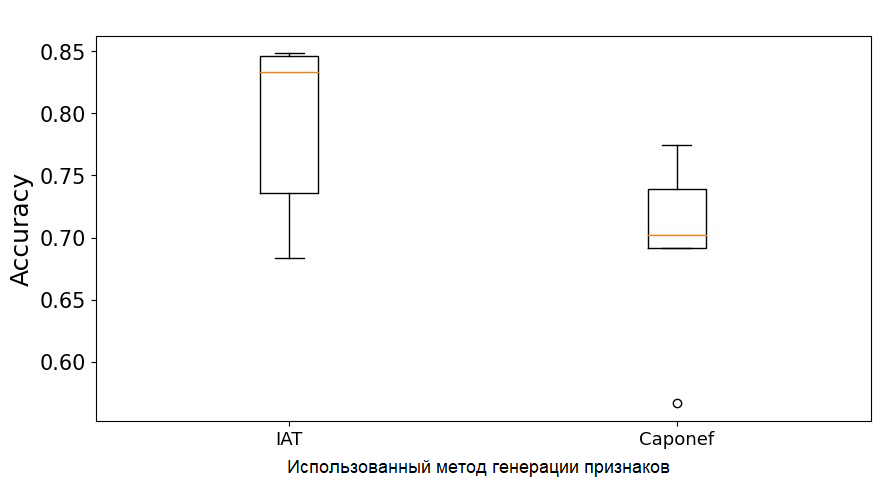
\includegraphics[width=0.9\linewidth]{images/caponef/RandomForest}
	\caption{Результаты использование CAPoNeF и алгоритма случайного леса для задачи бинарной классификации набора данных ISCXVPN}
	\label{fig:randomforest}
\end{figure}
\end{comment}

\begin{figure}[ht]
	\centering
	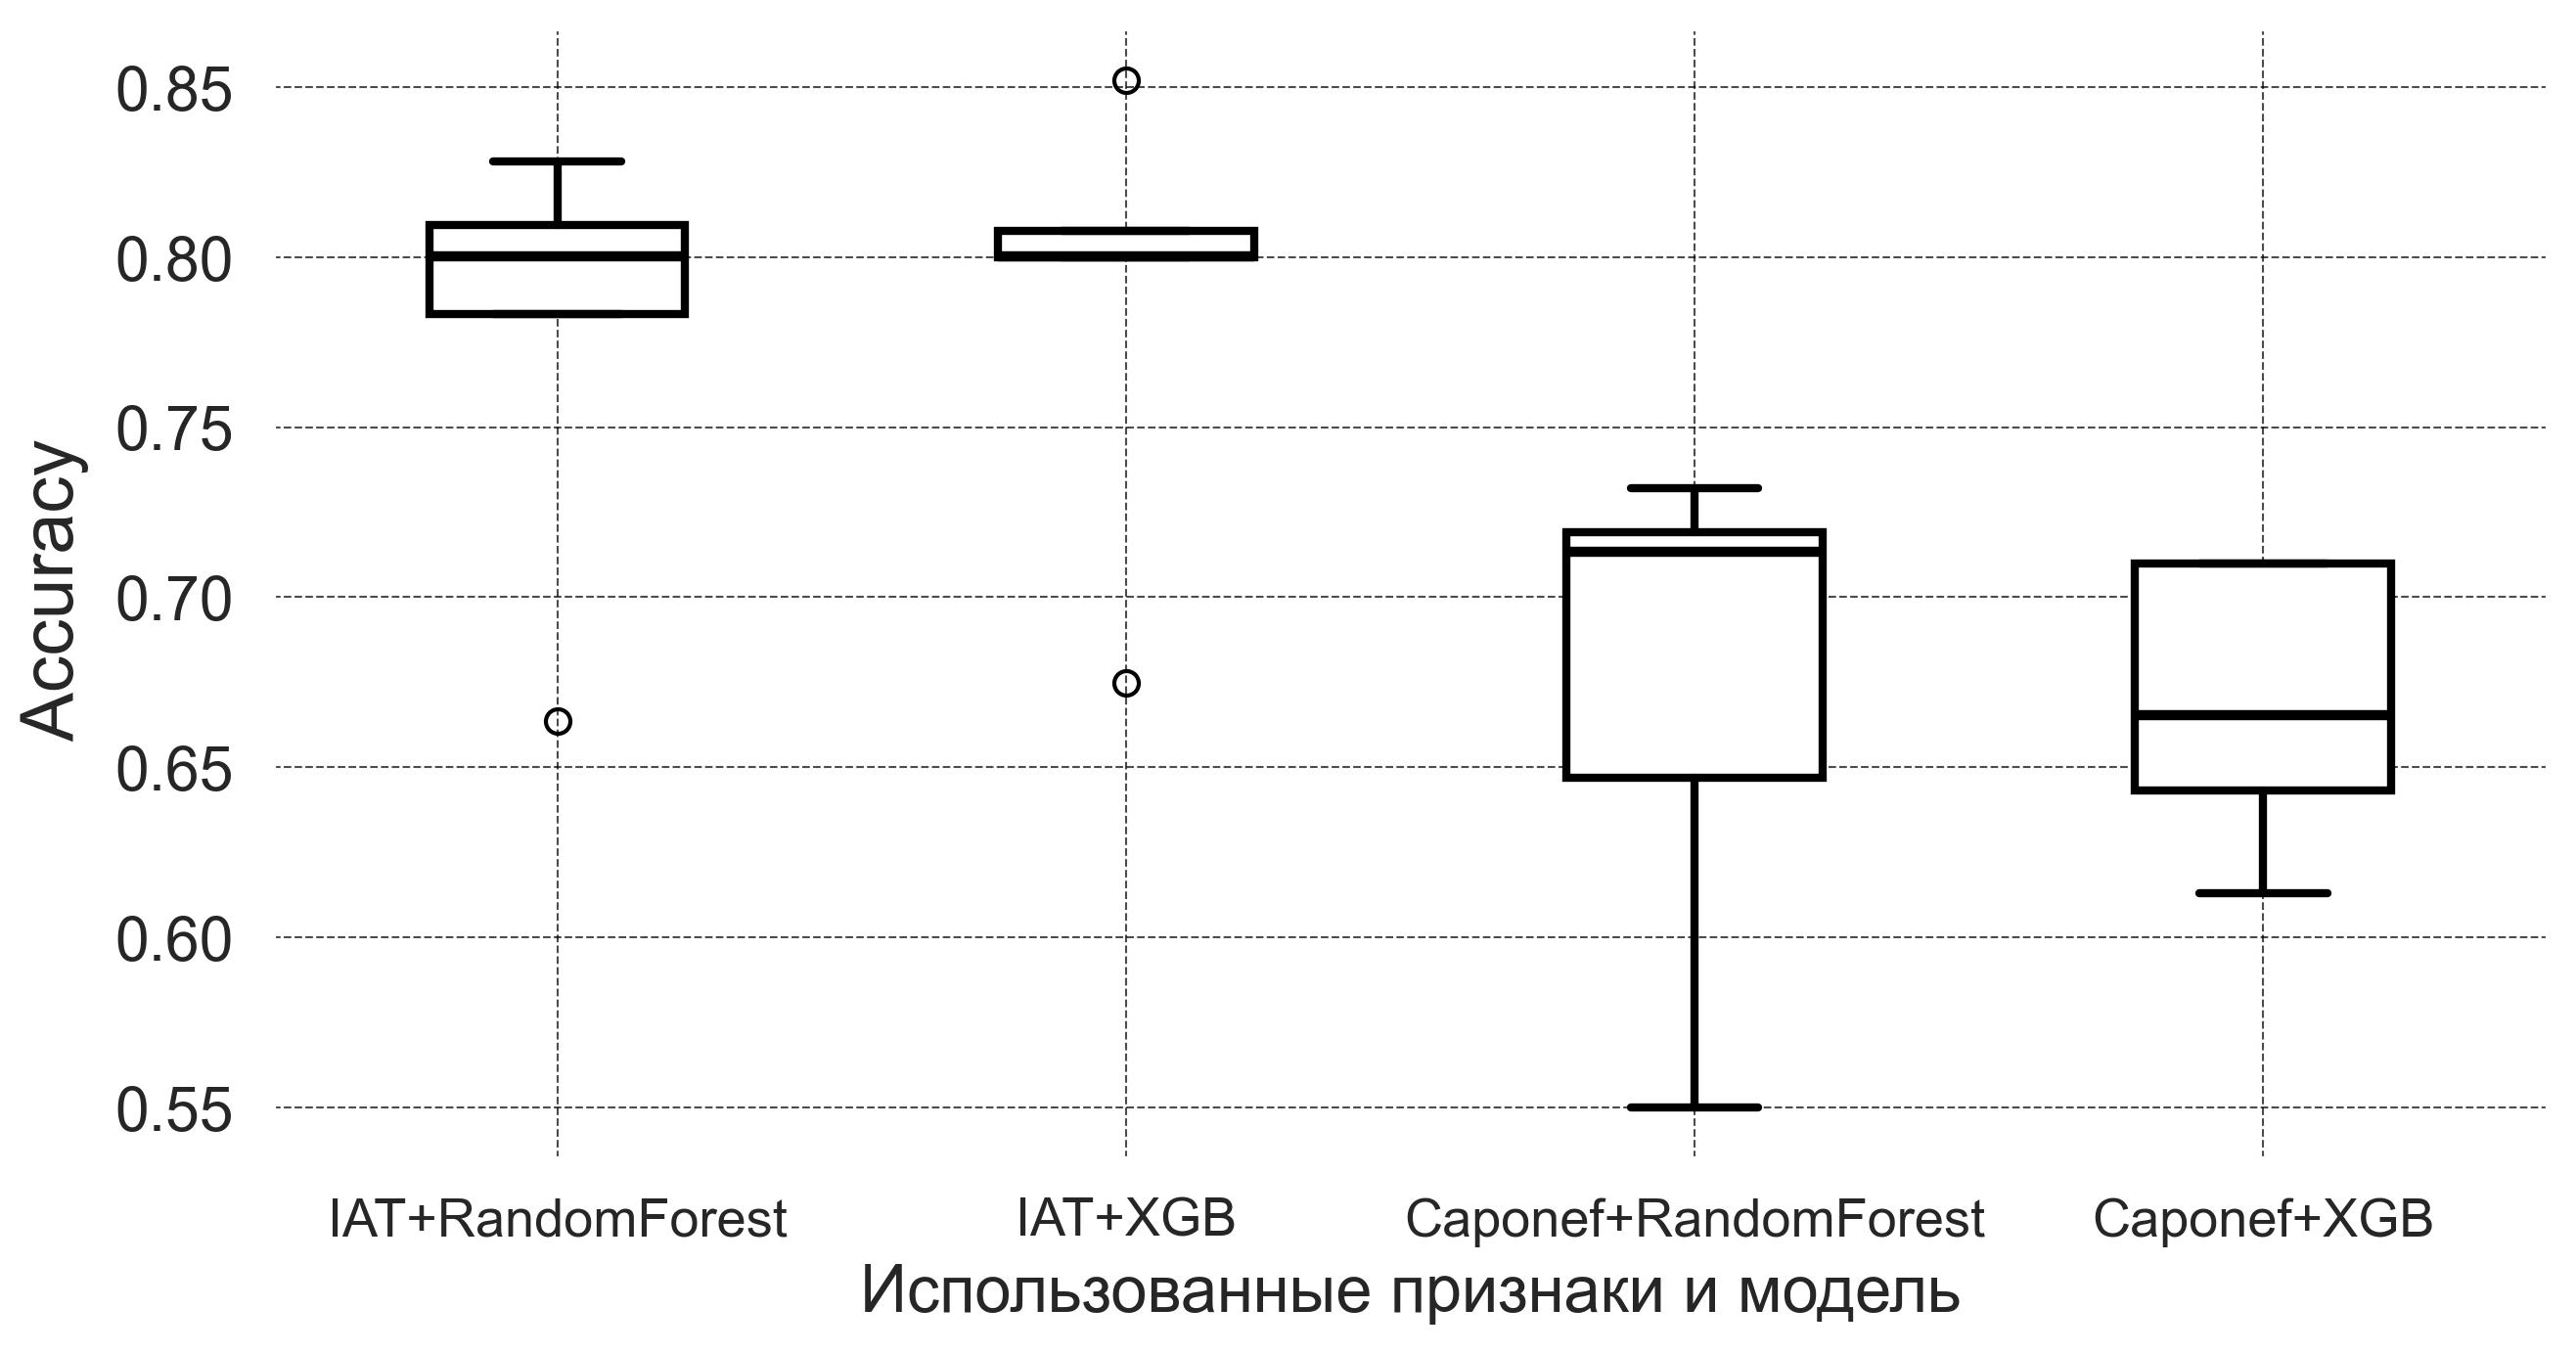
\includegraphics[width=0.7\linewidth]{images/caponef/iat_vs_cap_var_ru_bw}
	\caption{Результаты применения метода генерации признаков (CAPoNeF) и базовых признаков (IAT) для алгоритмов случайного леса(Randomforest) и градиентного бустинга(XGB)}
	\label{fig:capo}
\end{figure}


\section{Выводы по результатам второй главы}\label{sec:ch2/sect3}

В данной главе была продемонстрирована эффективность применения методов AGMV И CapoNef к предварительной обработке признаков для данных из датасетов ISCXVPN и CCCS-CIC- AndMal. В ходе проводимой обработки извлекалась дополнительная информация из природы временных рядов в качестве признаков с помощью AGMV. Было проведено сравнение и анализ производительности 4 классических ML-моделей (Таблицы \ref{vpn_res}, \ref{male_res}, \ref{male_pr_rc}).

% As it was shown, AGMV allow to reach over 0.95 accuracy in both tasks: binary traffic classification and malware categorization. We reached similar results as in State of the Art, but also some models showed better performance. But we should improve all metrics, especially sensitive to some anomalies in data such a class disbalance, for example. So we are going to improve Precision, Recall, and also research other metrics in further works.

Как было показано, AGMV позволяет достичь значений метрики accuracy более 0,95 как для задачи бинарной классификации на данных трафик, так и для задачи мультиклассовой классификации по оценке категории вредоносного ПО. Применяя данный метод, удалось достичь результатов, сравнимых с передовыми методами, а в некоторых сценариях метод показал себя даже лучше. Однако необходимо улучшить все метрики, особенно чувствительные к некоторым аномалиям в данных, таким как дисбаланс классов. Поэтому в дальнейшем исследовании будет проводиться улучшение метрик precision и recall, а также исследовать другие метрики.

Также хочется отметить, что в данной работе нет сравнения скорости обработки данных с другими методами, однако исследуемый подход должен быть быстрее, чем DNN, что уже облегчает использование данного подхода на маломощных устройствах, однако для сравнения с другими методами необходимо провести более подробное исследование.

Применение метода CAPoNeF привело к систематическому ухудшению результатов, что может указывать на чувствительность метода к параметрам или
ограничения его исходной концепции в условиях постановки задачи анализа трафика.

В заключении стоит отметить, что основной результат заключается в критическом переосмыслении ранее предложенных решений и их эмпирической проверке за пределами оригинальных условий. Получилось расширить область применения метода AGMV, а для CAPoNeF выявить границы применимости на основе экспериментального анализа. Полученные выводы могут быть использованы для более осознанного выбора стратегий генерации признаков в практических задачах анализа
данных и развития автоматизированных систем построения моделей.

\FloatBarrier
